% Zichen Tian

%%%%%%%%%%%%%%%%%%%%%%%%%%  configuration  %%%%%%%%%%%%%%%%%%%%%%%%%%
\documentclass{osa-article}
\journal{oe}

\usepackage{booktabs}
\usepackage[flushleft]{threeparttable}
\usepackage{fancyhdr}

\fancyhf{}
\renewcommand{\headrule}{}
\fancyfoot[R]{\thepage}
\pagestyle{fancy}

%%%%%%%%%%%%%%%%%%%%%%%%%%  author and abstract  %%%%%%%%%%%%%%%%%%%%%%%%%%
\begin{document}
\title{Report Title}
\author{Zichen Tian\authormark{1}\authormark{*}}
\address{\authormark{1}School of Electrical and Electronic Engineering, Nanyang Technological University, 50 Nanyang Avenue, 639798, Singapore}
\email{\authormark{*}ztian002@e.ntu.edu.sg} %% email address is required

\begin{abstract*}
There needs to be a summary of the major points, conclusions, and recommendations. It needs to be short as it is a general overview of the report. Some people will read the summary and only skim the report, so make sure you include all the relevant information. It would be best to write this last so you will include everything, even the points that might be added at the last minute.
\end{abstract*}

%%%%%%%%%%%%%%%%%%%%%%%%%%  body  %%%%%%%%%%%%%%%%%%%%%%%%%%
\section{Introduction}
The report needs to have an introduction. You will explain the problem and show the reader why the report is being made. You need to give a definition of terms if you did not include these in the title section, and explain how the details of the report are arranged. Example of reference~\cite{gallo1999all, masters1998three}, and~\cite{Yelin:03}

\section{Main Body}

This is the main section of the report.  There needs to be several sections, with each having a subtitle.  Information is usually arranged in order of importance with the most important information coming first.
All figure captions should be centered beneath the figure. Longer figure captions should be centered beneath the figure and alignment double (left and right) justified, but are not to exceed the left and right edge of the figure by more than 0.5 in. The abbreviation “Fig.” for figure should appear first followed by the figure number and a period. Captions should be in 8- pt. font. At least one line of space should be left before the figure and after the caption.


\begin{figure}[h!]
\centering
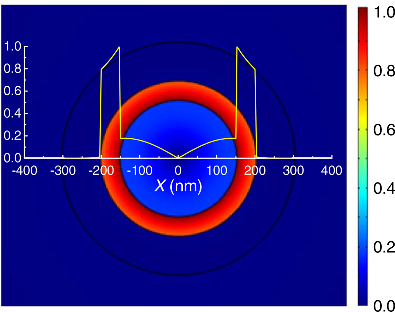
\includegraphics[width=0.6\textwidth]{osafig1.pdf}
\caption{Sample caption (Fig. 2, \cite{Yelin:03}).}
\end{figure}

Tables should be centered and numbered consecutively. Authors must use Word’s Table editor to insert tables. Authors must not import tables from Excel. All content for each table should be in a single Word table (do not split content for a single table across multiple Word tables). Tables should use horizontal lines to delimit the top and bottom of the table and column headings. Detailed explanations or table footnotes should be typed directly beneath the table, but not in a table cell. Table footnote labels should be alphabetical; numbers or special characters are not permitted. Position tables as closely as possible to where they are mentioned in the main text.

\begin{table}[ht]
\centering
\footnotesize
    \begin{threeparttable}
    \caption{Optical Constants of Thin Films of Materials\textsuperscript{a}}
    \label{tab:optical}
        \begin{tabular}{@{}llllll@{}}
            \toprule
                     & 83.4 nm &        &  & 121.6 nm &        \\ \cmidrule(lr){2-3} \cmidrule(l){5-6} 
            Material & n       & K      &  & n        & K      \\ \midrule
            Ir       & 1.182   & 0.865  &  & 1.450    & 1.040  \\
            MgF2     & 1.584   & 0.487  &  & 1.682    & 0.0627 \\
            Al       & 0.09874 & 0.1915 &  & 0.0424   & 1.137  \\
            Mo       & 0.98    & 1.08   &  & 0.78     & 1.03   \\
            C        & 1.16    & 1.29   &  & 1.85     & 1.10   \\ \bottomrule
        \end{tabular}
        \begin{tablenotes}
            \item \textsuperscript{a}Table source: Appl. Opt. \textbf{40}, 1128 (2001)~\cite{larruquert2001multilayer}.
        \end{tablenotes}
    \end{threeparttable}
\end{table}

\section{Conclusion}
This is where everything comes together. Keep this section free of jargon as most people will read the Conclusion.

%%%%%%%%%%%%%%%%%%%%%%% References %%%%%%%%%%%%%%%%%%%%%%%%%
\bibliography{ref}

\end{document}
